\chapter{Fonctionnement et tests}

Dans cette partie nous chercherons à décrire dans un premier temps les fonctionnements, ou, le cas échéant, les non fonctionnements de notre application.  Nous aborderons ensuite la politique de tests effectuée pour vérifier notre code. 

\section{Fonctionnement}

Lorsque l'on lance l'application, on exécute l'interface graphique. Cette interface fait appel aux autres parties de l'architecture pour afficher et organiser ses composants.

\subsection{Interface Graphique (GUI)}\label{GUI}

Tout d'abord, nous allons expliquer notre choix de technologie, qui s'est orienté vers le \textit{JavaFX}.
Nous pensions dans un premier temps développer l'application en \textit{Java} et générer des pages \textit{HTML} pour l'interface graphique. Puis après des recherches, nous avons découvert le \textit{JavaFX}, qui nous permettait de créer une interface graphique, mais à l'instar de la libraire \textit{Swing}, complètement personnalisable. Nous avons alors choisi ce langage afin d'avoir une application 100\% \textit{Java}.


La méthode \textit{main} de Start.java est appelée lors du démarrage de l'application. Cette méthode fait créé une instance de UserGUI, la première page de l'application qui s'affiche.

\begin{figure}[!ht]
\begin{center}
  \fbox{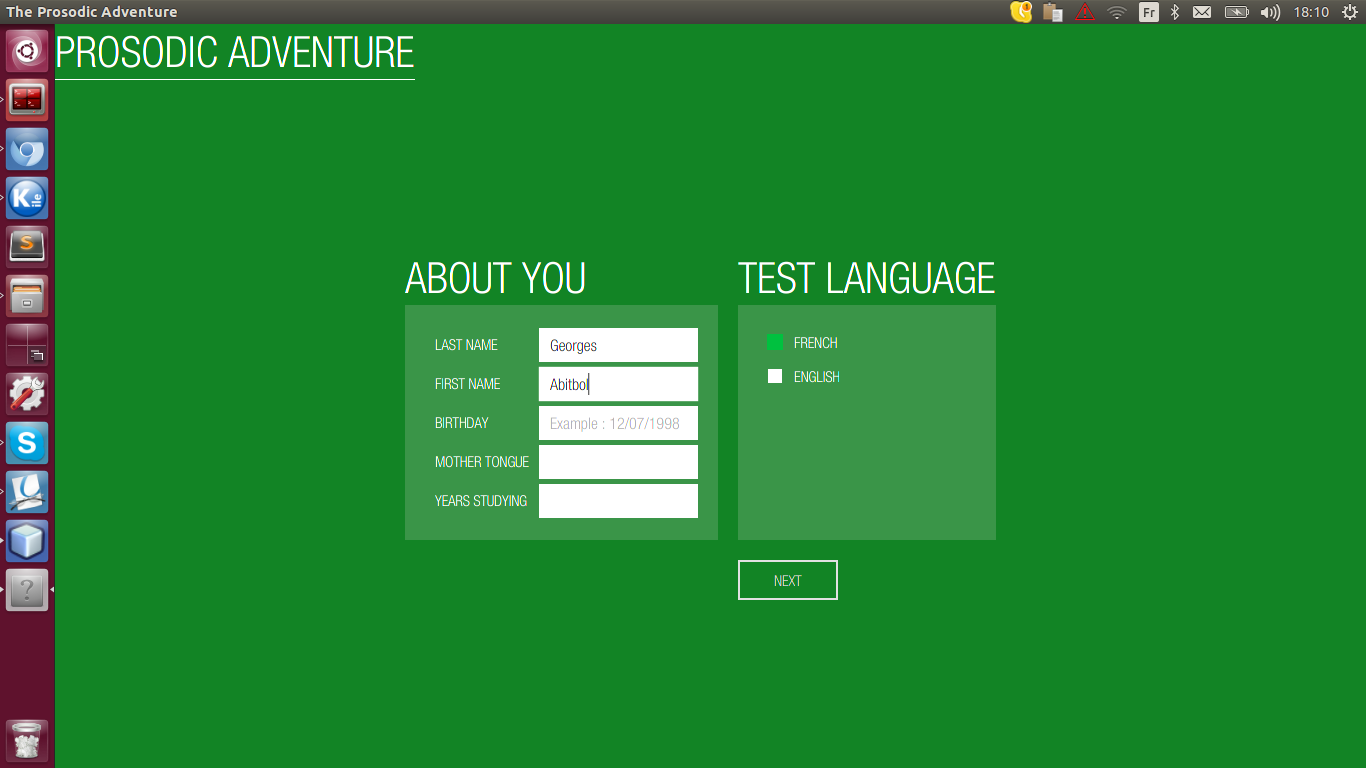
\includegraphics[width=8cm]{./fonctionnement_tests/UserGUI.png}}
  \caption{Fonctionnement - UserGUI}
  \label{UserGUI} 
\end{center}
\end{figure}

Pour récupérer les langues disponibles, UserGUI fait appel au contrôleur, dont nous décrirons le fonctionnement par la suite.
Les informations entrées par l'utilisateur dans les champs de ``\textsc{about you}'' (voir \textsc{Figure} \ref{UserGUI}) sont récupérés lors du clic sur le bouton ``\textsc{next}''. Ces données sont récupérées dans un fichier \textit{txt} par le biais du package \textit{Extract} que nous allons voir plus tard.

Après l'exportation des données sur l'utilisateur, un lien est fait vers la seconde page de l'interface : ChooseGUI (voir \textsc{Figure} \ref{ChooseGUI}). Cette page est une simple page avec deux boutons pour savoir dans quel mode veut aller l'utilisateur (apprentissage da l'application ou test concret).

\newpage

\begin{figure}[!ht]
\begin{center}
  \fbox{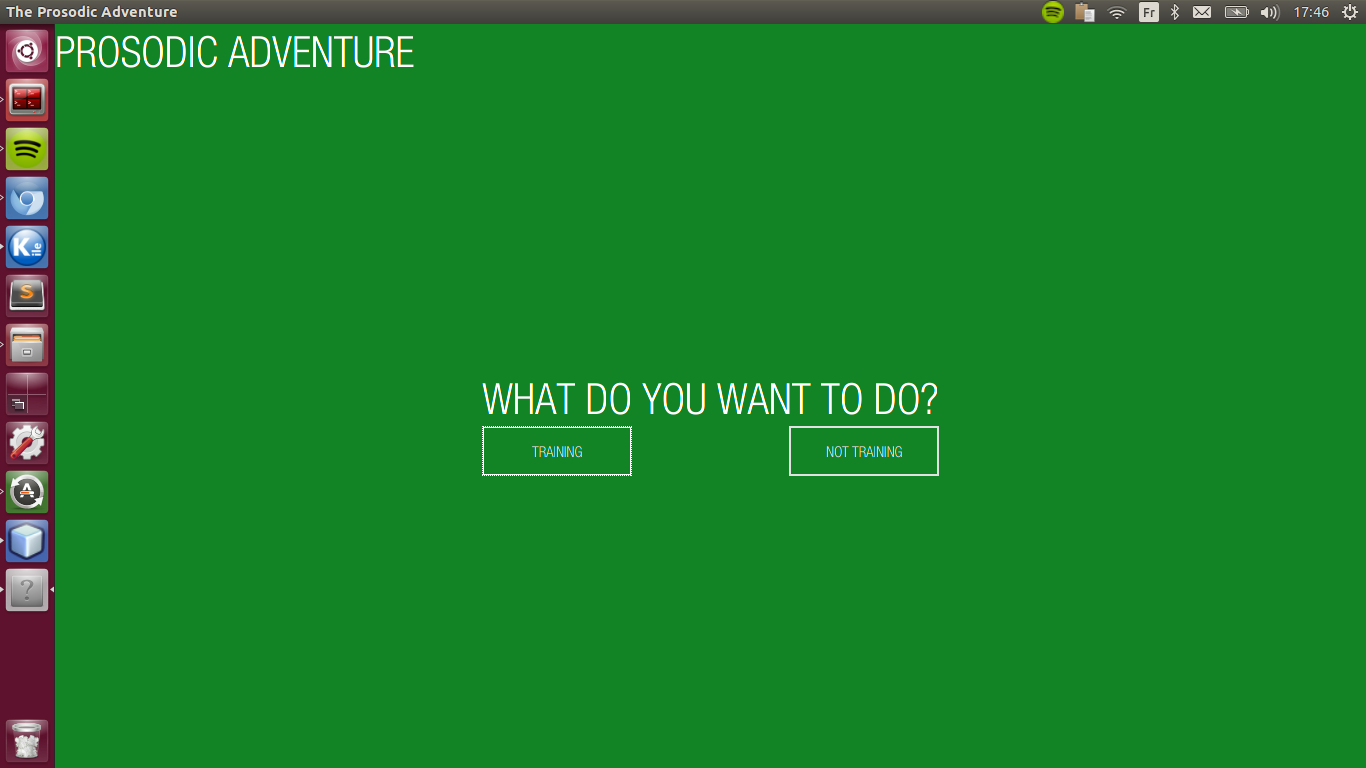
\includegraphics[width=8cm]{./fonctionnement_tests/ChooseGUI.png}}
  \caption{Fonctionnement - ChooseGUI}
  \label{ChooseGUI} 
\end{center}
\end{figure}

On est ensuite dirigé vers le page de test (identique dans le mode ``\textsc{training}'' et ``\textsc{not training}''). La seule différence entre les deux mode est l'exportation de données : dans le test réel, les données sont exportées tandis que dans le mode de découverte, rien n'est exporté.
Les données exportées sont :
\begin{itemize}
 \item Les questions posées
 \item La vidéo réponse
 \item L'audio réponse
\end{itemize}
Ces données sont exportées lors du clic sur le bouton ``\textsc{next}''.

\begin{figure}[!ht]
\begin{center}
  \fbox{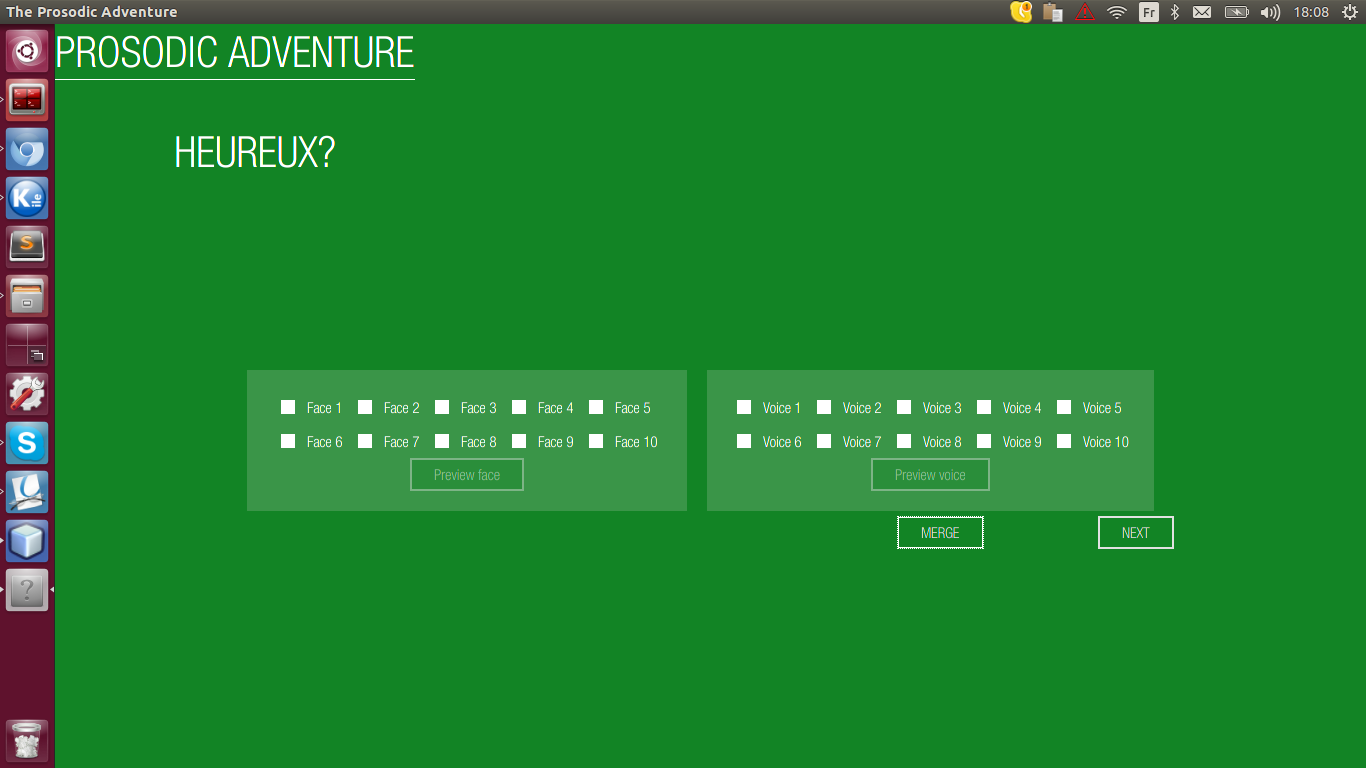
\includegraphics[width=8cm]{./fonctionnement_tests/TestGUI.png}}
  \caption{Fonctionnement - TestGUI}
  \label{ChooseGUI} 
\end{center}
\end{figure}

Les boutons ``\textsc{preview}'' permettent de voir le contenu des vidéos et d'écouter les sons disponibles dans les différentes listes. Afin d'être joués, les médias sont ouverts (voir \textsc{Figure} \ref{VLC} avec VLC (en \textit{standalone}) en faisant appel à la librairie VLC inclue dans le projet.

\begin{figure}[!ht]
\begin{center}
  \fbox{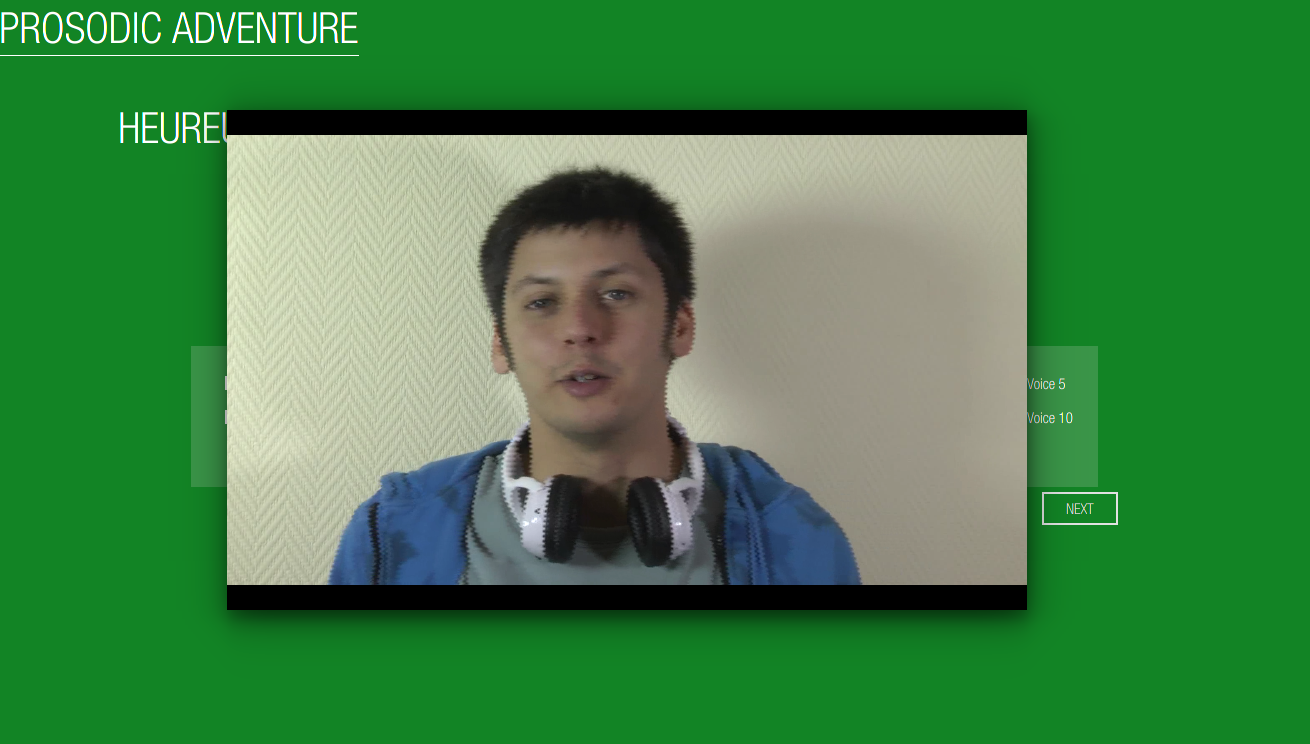
\includegraphics[width=8cm]{./fonctionnement_tests/VLC.png}}
  \caption{Fonctionnement - TestGUI}
  \label{VLC} 
\end{center}
\end{figure}

Finalement, une fois le test terminé, l'utilisateur est redirigé vers une page terminal contenant juste un message de remerciements, ainsi qu'un bouton ramenant vers la première page (\textit{UserGUI}).

\begin{figure}[!ht]
\begin{center}
  \fbox{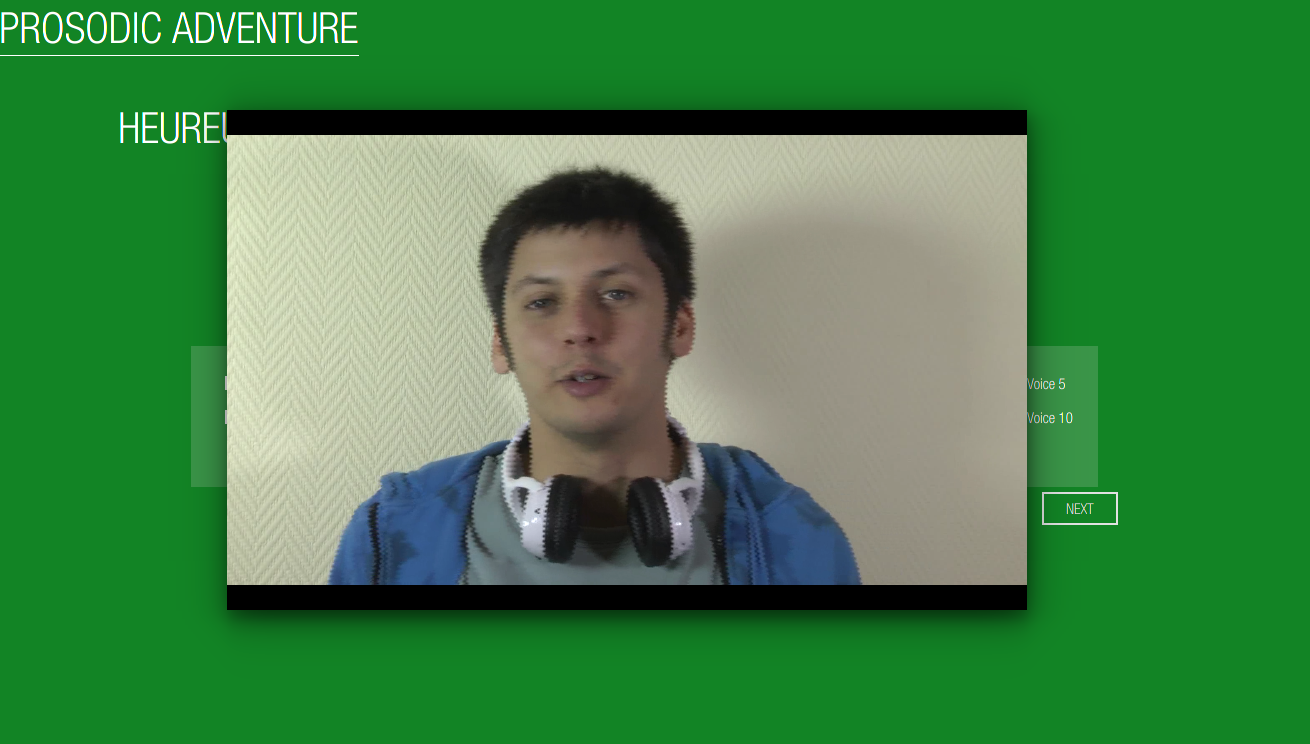
\includegraphics[width=8cm]{./fonctionnement_tests/VLC.png}}
  \caption{Fonctionnement - EndGUI}
  \label{VLC} 
\end{center}
\end{figure}

\subsection{Base de données}\label{BDD}

Le système de gestion de base de données relationnelles (SGBDR) choisi a été \textit{SQLite}. Ce SGBDR est utilisable sur n'importe quelle plateforme, sans nécessiter l'installation et la mise en place d'un serveur, il se résume à un fichier \textit{.db} qui contient toute la base de données.
Pour le fontionnement de l'application, des méthodes d'accès à la base de données ont été necessaires à implémenter :


\begin{itemize}
 \item Création de la base de données et de ses dépendances (si elle n'existe pas)
 \item Remplissage de la base de données
 \item Consultation du contenu de la base de données
 \item Recherche dans la base de données selon plusieurs critères
 \item Tirage au hasard d'un media de la base de données
 \item Suppression d'un media de la base de données, tout en vérifiant l'intégrité des relations (voir exemple plus en fin du paragraphe suivant)
\end{itemize}


Toutes ces implémentations sont fonctionnelles. Des tests ont été réalisés dessus (voir \ref{tests}).
Les accès à la base de données sont effectués par le driver\footnote{sqlite-jdbc-3.8.7} \textit{Java} de \textit{SQLite}.

Pour éviter tout conflit lors de l'accès à la base de données, des transactions manuelles ont été mises en place : un verrou est créé à chaque accès, ainsi un double accès ne peut pas être effectué.
Etant donné que \textit{SQLite} ne gère pas les contraintes de clef étrangère, nous avons établi un système de vérification en \textit{Java}. Cette vérification vérifie avant chaque modification sensible (suppression d'une vidéo qui pourrait être liée à une question par exemple), qu'aucune dépendance ne sera brisée.


\subsection{Contrôleur}\label{controller}



Pour ce faire, nous avons mis en place un package controleur se composant de trois classes :

\begin{itemize}
  \item \textsc{ControllerDatabase}: Permettant de générer la base de données si elle n'existe pas et d'obtenir les langages disponibles
  \item \textsc{MediaSelected}: Permettant de récupérer les réponses de l'utilisateur et de les stocker.
  \item \textsc{SelectMedia}: Permettant la sélection et le choix de media.
\end{itemize}

Détaillons un peu plus ces classes :

\textsc{ControllerDatabase}:Les fonctions contenues dans cette classe retournent des données(audios/videos/questions) et le compte de ces dites données.
\textsc{MediaSelected}: Les fonctions contenues dans cette classe retournent des données(utilisateurs/languages) de la base de données existantes et la liste des réponses, liste de réponses que nous pouvons agrémenter grace à la fonction \textit{addAnswer(Answer)}.
\textsc{SelectMedia}:Les fonctions contenues dans cette classe permettent dans un premier temps à générer des listes stockant les éléments de la base de données, puis dans un second temps d'effectuer une sélection dans les listes créées précédemment.

Toutes ces fonctions sont par la suite appelées dans le package GUI (voir \ref{GUI}) pour ainsi effectuer le lien avec la base de données.

\subsection{Exportation des données}\label{export}

Tout ce qui concerne l'exportation des données se situe dans le package \textit{Result}. Ce package est séparé en 
 éléments :
 
 \begin{itemize}
  \item \textit{Answer.java} qui permet de créer un objet \textit{Answer} afin centraliser les données à extraire.
  \item \textit{User.java} qui a la même fonction que la classe précédente, mais qui contient les informations sur l'utilisateur (informations récupérées dans l'interface \textit{UserGUI}, voir \ref{GUI}).
  \item \textit{Extract} extrait les données contenues dans les deux précédents types d'objet, et les écrit dans un fichier texte, comme dans l'exemple suivant :
 \end{itemize}
 
 \begin{verbnobox}[\small]
  Langage:   French
  User:
      First Name:   Georges
      Last Name:   Abitbol
      Birthday   09/08/1979
      Mother Tongue   French
      Years learning tongue selected   1
  List of answers
      Answer 1:
	    Question:   Pouvez-vous exprimer la douleur avec ces audios et vidéo ?
	    Video   2013_3_19_S29_fr_L1_ADMI_B_ok
	    Audio   wasted
      Answer 2:
	    Question:   Pouvez-vous exprimer le bonheur avec ces audios et vidéo ?
	    Video   2013_3_19_S29_fr_L1_ADMI_B_ok
	    Audio   wasted
      Answer 3:
	    Question:   Pouvez-vous exprimer la passion avec ces audios et vidéo ?
	    Video   2013_3_19_S29_fr_L1_ADMI_B_ok
	    Audio   mark
      Answer 4:
	    Question:   Pouvez-vous exprimer la séduction avec ces audios et vidéo ?
	    Video   2013_3_19_S29_fr_L1_ADMI_B_ok
	    Audio   mark
      Answer 5:
	    Question:   Pouvez-vous exprimer l'exaltation avec ces audios et vidéo ?
	    Video   2013_3_19_S29_fr_L1_ADMI_B_ok
	    Audio   mark

 \end{verbnobox}



\section{Tests}\label{tests}

\subsection{JUnit}

Pour réaliser les tests unitaires sur la base de données, nous avons utilisé le plugin \textit{JUnit}, disponible par défaut dans l'IDE \textit{Netbeans}.
Ce plugin permet de tester chaque méthode, afin de détecter d'éventuels problèmes d'implémentation.

\subsection{Performances}

Afin de réaliser les tests de performance, nous avons simplement utilisé un plugin de \textit{Netbeans}. Ce plugin permet de mesurer les performance en temps réel.

Sachant déjà que nous avions un problème de performance pendant le chargement de la page \textit{TestGUI} (voir \ref{GUI}), ce test nous a permis d'identifier le code fautif.
Ainsi, l'accès à la base de données a été mis en cause. La méthode de connexion étant seulement gérée par le driver \textit{SQLite-jdbc}, nous pouvons nous affranchir de tout problème de lenteur dans notre code actuel. Cependant, ce point permet d'envisager une future amélioration à ce niveau là, en déployant un SQGB plus efficace pour notre utilisation.


\subsection{Tests boite blanche}



\subsection{Test de recouvrement}